\documentclass[11pt]{beamer}
\usepackage{amsfonts,amssymb, amsmath,amsthm,mathrsfs, tikz,pgfplots}
\usepackage{array}

\usetheme{eaperry}
%\usetheme{CoeCollege}

%\bibliographystyle{aer}
\usepackage{natbib}

\title{A Theory of Investment for\\ Energy-Efficient Technologies}
\subtitle{Part IV}
\author{Evan Perry}
\institute{Spellman Program}
\date{July 6, 2021}

\begin{document}

\maketitlepage

\begin{frame}{Review}

\begin{exampleblock}{\large\textbf{Research Question}}
What neighborhood characteristics relate to the number of certified energy-efficient commercial buildings?
\end{exampleblock}

\vfill
Previously:
\begin{itemize}
	\item Energy Savings v. Adoption Costs
	\item Premium on Green Buildings
	\item We still need an explicitly spatial link to the adoption decision
\end{itemize}
\end{frame}

\begin{frame}{Paper}

%{\bf Wiley, Jonathan~A, Justin~D Benefield, and Ken~H Johnson},\\
%\quad  ``Green design and the market for commercial office space,'' {\it The\\
%\quad  Journal of Real Estate Finance and Economics}, 2010, {\it 41} (2),\\ 
%\quad 228--243.\\
%
%{\bf Alonso, William}, {\it Location and land use}, Harvard University Press,\\
%  \quad 1964.

{\bf Brueckner, Jan~K}, {\it Lectures on urban economics}, MIT press,\\
\quad 2011.

\vfill
\begin{itemize}
	\item Develops the \cite{alonso2013location}, \cite{muth1969cities}, \cite{mills1967aggregative} (AMM) Model
	
	\vfill
	\item Why the AMM Model?
	\begin{itemize}
		\item Fundamental urban model
		\item Empirically supported
		\item Allows us to consider how different agents locate themselves within a city
	\end{itemize}
%	\item Create a model to address:
%	\begin{itemize}
%		\item How much housing to buy?
%		\item How much to pay for housing?
%		\item Where to buy housing?
%	\end{itemize}
	\vfill
	
	\item Modify this model to consider location of different types of developers
\end{itemize}

\end{frame}





\begin{frame}{Overview}

\begin{description}
	\item[Purpose] Within a city, where will developers construct green buildings?
	\vfill
	
	\item[Context] The AMM Model
	\vfill
	
	\item[Model] Modify the AMM model with a green developer and non-green developer
	\vfill
	
	\item[Results] Green buildings cluster away from the city center
\end{description}

\end{frame}


\newsection{Context}{\textit{An Overview of the Alonso-Muth-Mills (AMM) Model}}


\begin{frame}{The AMM Model Environment}

\begin{itemize}
	\item Many identical agents need to purchase housing
	
	\vfill
	\item Live in a  linear city: pick a distance from the city center and purchase housing there
	\vspace{.5cm}
	\begin{center}
	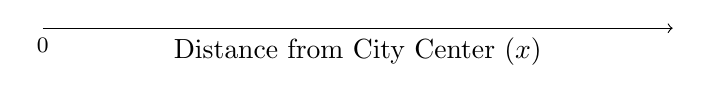
\begin{tikzpicture}
		\draw[->] (0,0) node[below]{\footnotesize 0} -- (8,0) node[below, pos = .5]{Distance from City Center $(x)$};
	\end{tikzpicture}
	\end{center}
	
	\vfill
	\item Everyone needs to commute to the city center and gets disutility from commuting
	\vfill
	
	\item Spatial Equilibrium Condition: the price of housing must adjust so identical agents are indifferent between locations 	
\end{itemize}

\end{frame}


\begin{frame}{The Bid-Rent Curve}

\begin{figure}
\centering
\caption{Baseline Bid-Rent Curve}
\begin{tikzpicture}
\begin{axis}[
	axis lines = left,
	ticks=none,
    ylabel = {Price of Housing/sq.ft. ($p_H$)},
    xlabel = {Distance from City Center ($x$)},
    xmin=0, xmax=7,
    ymin=0, ymax=10,
	every axis plot/.append style={ultra thick}
]
\addplot[
	domain = 0.1:6,
	samples=100,
	color=EAPred
]{.7*(.3/1)^(.7/.3)*((5 - 0.5*x)/1)^(1/.3)};
\end{axis}
\node[EAPred, right] at (6,0.25) {$p_H$};
\end{tikzpicture}
\end{figure}

\end{frame}


\begin{frame}{Two Important Takeaways}

\begin{enumerate}
	\item Quantity of housing each agents purchases increases as we move away from the city center
	\vfill
	
	\item Rent per sq.ft. decreases as we move away from the city center
\end{enumerate}

\end{frame}


\newsection{Model}{\textit{Modifying the Alonso-Muth-Mills (AMM) Model}}


\begin{frame}{Two Developers: Green \& Non-Green}

$$Q = A M_i^\alpha L^\beta \hspace{2cm} C = p_{M_i} M_i + p_L L$$

\vfill
\footnotesize
\begin{itemize}
	\item $Q$ : Commercial Space (in sq. ft.)
	\item $C$ : Cost 
	\item $A$ : Technology Index
	\item $M_i$ : Materials of type $i$
	\begin{itemize}
		\item $G$ : Green Materials
		\item $N$ : Non-Green Materials
	\end{itemize}
	\item $p_{M_i}$ : Price of Materials of type $i$
	\begin{itemize}
		\item We say $p_{M_G} > p_{M_N}$
	\end{itemize}
	\item $L$ : Land (in sq. ft.)
	\item $p_L$ : Price of Land (in \$/sq. ft.)
\end{itemize}

\end{frame}

\begin{frame}{Demand for Space}

Green developers can sell their output for a higher price: 

$$p_G = p_N + r$$

where $r$ is the premium for green space.
\end{frame}


%\begin{frame}{Model Primitives}
%\begin{columns}
%\begin{column}{0.3\linewidth}
%\centering
%\textbf{Production}
%
%$$Q_G = A M_G^\alpha L^\beta$$
%$$Q_N = A M_N^\alpha L^\beta$$
%
%\bigskip
%$$\textcolor{white}{t}$$
%
%\end{column}
%\begin{column}{0.3\linewidth}
%\centering
%\textbf{Costs}
%
%$$C = p_{M_G} M_G + p_L L$$
%$$C = p_{M_N} M_N + p_L L$$
%
%\bigskip
%$$p_{M_G} > p_{M_N}$$
%
%\end{column}
%\begin{column}{0.3\linewidth}
%\centering
%\textbf{Demand}
%
%$$Q(x)  = (b - cx)^{-1}$$
%$$p_{Q_N}(x) = a(b - cx)^{2}$$
%
%\bigskip
%$$p_{Q_G} = p_{Q_N} + r$$
%\end{column}
%\end{columns}
%\end{frame}


\begin{frame}{The Derivation}

\begin{enumerate}
	\item For a representative developer, derive its profit functions for green and non-green construction
	\vfill
	
	\item For several identical developers, impose spatial equilibrium and solve for their bid-rent curves
	\vfill
	
	\item Use the bid-rent curves to identify where green and non-green construction happens
\end{enumerate}


\end{frame}


\newsection{Results}{}


\begin{frame}{Land Intensity}

\begin{figure}
\centering
\caption{Bid-Rent Curves without a Premium}
\begin{tikzpicture}
\begin{axis}[
	axis lines = left,
	ticks=none,
    ylabel = {Price of Land ($p_L$)},
    xlabel = {Distance from City Center ($x$)},
    xmin=0, xmax=10,
    ymin=0, ymax=15,
	every axis plot/.append style={ultra thick}
]
\addplot[
	domain = 0.1:10,
	samples=100,
	color=EAPred
]{(1/(100000*(10-0.2*x)^(-1)))^(1/0.4) * (0.6/(0.4*10))^(0.6/0.4) * 
       (0.4/(1))^((1)/0.4)*(50000*(10 - 0.2*x) - 10000 - 265750)^((1)/0.4)};
\addplot[
	domain = 0.1:10,
	samples=100,
	color=EAPgreen
]{(1/(100000*(10-0.2*x)^(-1)))^(1/0.4) * (0.6/(0.4*20))^(0.6/0.4) * 
       (0.4/(1))^((1)/0.4)*( 
       (50000*(1/100000)*(10 - 0.2*x)^(1+1))*100000*(10-0.2*x)^(-1)
         - 10000 - 265750)^((1)/0.4)};
\end{axis}
\node[EAPgreen] at (7.2,0.2) {$p_L^G$};
\node[EAPred] at (7.2,0.8) {$p_L^N$};
%\draw[dashed]  (3,0) -- (3,5.4);
%\node[EAPred] at (1.5, 1) {\footnotesize Non-Green};
%\node[EAPgreen] at (4.5, 1) {\footnotesize Green};
%\node at (5.1, 5) {\footnotesize $\Delta p KWH > \Delta \psi \rho$};
\end{tikzpicture}
\end{figure}

\end{frame}



\begin{frame}{Green and Non-Green Sorting}

\begin{figure}
\centering
\caption{Bid-Rent Curves with a Fixed Premium}
\begin{tikzpicture}
\begin{axis}[
	axis lines = left,
	ticks=none,
    ylabel = {Price of Land ($p_L$)},
    xlabel = {Distance from City Center ($x$)},
    xmin=0, xmax=10,
    ymin=0, ymax=15,
	every axis plot/.append style={ultra thick}
]
\addplot[
	domain = 0.1:10,
	samples=100,
	color=EAPred
]{(1/(100000*(10-0.2*x)^(-1)))^(1/0.4) * (0.6/(0.4*10))^(0.6/0.4) * 
       (0.4/(1))^((1)/0.4)*(50000*(10 - 0.2*x) - 10000 - 265750)^((1)/0.4)};
\addplot[
	domain = 0.1:10,
	samples=100,
	color=EAPgreen
]{(1/(100000*(10-0.2*x)^(-1)))^(1/0.4) * (0.6/(0.4*20))^(0.6/0.4) * 
       (0.4/(1))^((1)/0.4)*( 
       (50000*(1/100000)*(10 - 0.2*x)^(1+1) + 8.5)*100000*(10-0.2*x)^(-1)
         - 10000 - 265750)^((1)/0.4)};
\end{axis}
\node[EAPgreen] at (7.2,1.2) {$p_L^G$};
\node[EAPred] at (7.2,0.6) {$p_L^N$};
\draw[dashed]  (3,0) -- (3,5.4);
\node[EAPred] at (1.5, 5) {\footnotesize Non-Green};
\node[EAPgreen] at (4.5, 5) {\footnotesize Green};
%\node at (5.1, 5) {\footnotesize $\Delta p KWH > \Delta \psi \rho$};
\end{tikzpicture}
\end{figure}

\end{frame}


\begin{frame}{Model Takeaways}

\textbf{\textcolor{EAPgreen}{Q :}} Within a city, where will developers construct green buildings?

\vfill
\textbf{\textcolor{EAPgreen}{A :}} Developers will build green buildings away from the city center
\begin{itemize}
	\item[\textcolor{EAPyellow}{$\blacktriangleright$}] Production becomes more land intensive / less material intensive away from the city center
	\item[\textcolor{EAPyellow}{$\blacktriangleright$}] Spaces are larger as we move away from the city center, meaning larger premiums
\end{itemize}


\end{frame}


\begin{frame}{Next Week}

Data Week
\begin{itemize}
	\item Energy Star \& LEED Database
	\item Initial Data Exploration
	\item Maps
\end{itemize}

\end{frame}


\begin{frame}{References}
\bibliographystyle{aer}
\bibliography{References}
\end{frame}


\newsection{Appendix}{\textit{Derivations and Important Equations}}

\begin{frame}{First-Order Conditions}

\begin{align*}
	\mathscr{L} &= p_i M_i + p_L L + k - \lambda( AM_i^\alpha L^\beta - \bar{Q})\\
	\mathscr{L}_M &= p_i - \alpha AM_i^{\alpha - 1} L^\beta = 0\\
	\mathscr{L}_L &= p_L - \beta AM_i^\alpha L^{\beta -1} = 0\\
	\mathscr{L}_\lambda &= \bar{Q} - AM_i^\alpha L^\beta = 0
\end{align*}

\end{frame}


\begin{frame}{Spatial Equilibrium Condition}

$$ \bar{\Pi} = p_i(x) \cdot Q(x) - C( Q(x) : p_i, p_L) $$

\end{frame}


\begin{frame}{The Bid-Rent Curve (Equation)}

\[
p_L^i(x) = \left( \frac{A}{Q(x)}\right)^{1/\beta} \left( \frac{1}{p_i}\right)^{\alpha/\beta} \Phi(\alpha, \beta) \left[ p_i(x)\cdot Q(x) - \bar{\Pi} \right]^{(\alpha + \beta)/\beta}
\]
\vfill
where $Q(x)  = (b - cx)^{-1}$, $p_N(x) = a(b - cx)^{2}$, and $p_G(x) = p_N(x) + r$. 
\vfill

$\Phi(\alpha, \beta)$ is a constant and $\bar{\Pi}$ is the common profit level of all developers.


\end{frame}


\end{document}